%&presentation.fmt
% !TEX program = pdflatex
% !BIB program = biber

% UNCOMMENT THIS WHEN NOT USING .fmt FILE OR WHEN GENERATING .fmt FILE
% %!TEX root = ./presentation.tex 
\scrollmode

\documentclass[aspectratio=169]{beamer}
\usetheme{Madrid}


% -------------- COMPILE VARIABLES --------------
\newif\ifINTRO

\INTROfalse      % Build only intro slide


% ------------------ VARIABLES ------------------
\newcommand{\userName}{Pascal-Emmanuel Lachance \&\\Maxime Grenier-Castillo}
\newcommand{\initials}{P-E.L \& M. G-C}
\newcommand{\projectName}{Comment se Propage un Signal Électro-Magnétique?}


% Le Parfait Petit Manuel Pluridisciplinaire et Multidisciplinaire
% Pour les PCB Multicouches Prototypables et Manufacturables
% Par Petit Maxime et Petit Pascal
% Par le Moyen d'une Présentation Procédurale PowerPoint Multimédia sur les PCB en Présentiel
% Pour les Misérables Pragmatiques

\newcommand{\institution}{C3i}
\newcommand{\repo}{PPPPP}
\newcommand{\user}{raesangur}
\newcommand{\docName}{Presentation}

\author{\userName}
\title{\projectName}
\subtitle{PPMPMPPMPMPPMPPPMPPPMPPPMP05}
\institute{Compétitions de Conception de Circuits Imprimés}
\date{\today}


% ----------- CONFIGURATION INCLUDES ------------
%!TEX root = ../presentation.tex

%%%%%%%%%%%%
% PACKAGES %
%%%%%%%%%%%%

% =============== General Formatting ============
\usepackage[T1]{fontenc}
\usepackage{lmodern}
\usepackage{pifont}
\usepackage{amsmath}
\usepackage{amssymb}
\usepackage{fontawesome5}
\usepackage{comment}
\usepackage{adjustbox}
\usepackage{array}
\usepackage{multicol}
\usepackage[yyyymmdd]{datetime}

% =============== Colors ============
\usepackage{colortbl}
\usepackage[many]{tcolorbox}
\usepackage{xcolor}
\usepackage{hyperref}

% =============== Math ============
\usepackage{mathtools}
\usepackage{nicefrac}
\usepackage{siunitx}
\usepackage{calc}

% =============== Figures ============
\usepackage{tikz}
\usepackage{circuitikz}
\usepackage{pgfplots}
\usepackage{animate}
\usepackage{environ}

% =============== Listings ============
\tcbuselibrary{listings}      % Raesangur
\usepackage{listings}         % Main package for inserting code
\tcbset{listing engine={listings}}
\usepackage[scaled]{beramono} % For using the beramono font


% =============== Bibliography ============
%\usepackage{cite}

\usepackage[style=alphabetic,backend=biber, style=numeric, sorting=none]{biblatex}
%\addbibresource{references.bib}
\renewcommand*{\mkbibacro}[1]{#1}




% =============== Package Setup ============
\newcolumntype{C}[1]{>{\centering\arraybackslash}p{#1}}

\renewcommand{\dateseparator}{--}

\newcommand{\cmark}{\ding{51}} % ✓
\newcommand{\xmark}{\ding{55}} % ✗


% ------ Tikz ------
\usetikzlibrary{arrows, shapes, calc, positioning}
%\usetikzlibrary{external}
%\usepgfplotslibrary{external}
%\tikzexternalize
\pgfplotsset{compat=1.18}
%!TEX root = ../presentation.tex


% -------------- BACKGROUNDS --------------

\newcommand\titlebackground {
    \usebackgroundtemplate{
    \begin{tikzpicture}[remember picture, overlay]
        \node[at=(current page.center)] {
            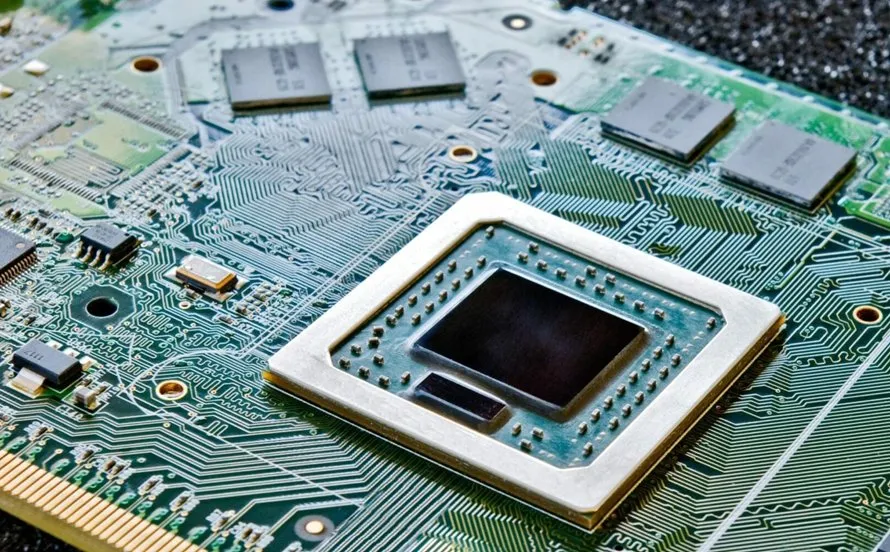
\includegraphics
            [width=\paperwidth, keepaspectratio]
            {pictures/background/background-PCB.png}
        };
    \end{tikzpicture}
    }
}


\newcommand\introbackground {
    \usebackgroundtemplate{
    \begin{tikzpicture}[remember picture, overlay]
        \node[at=(current page.center)] {
            
\includegraphics
            [width=\paperwidth, keepaspectratio]
            {pictures/background/background-pcb-poster.png}
        };
    \end{tikzpicture}
    }
}

\newcommand\defaultbackground {
    \usebackgroundtemplate{
    \begin{tikzpicture}[remember picture, overlay]
        \node[at=(current page.center)] {
            
\includegraphics
            [width=\paperwidth, keepaspectratio]
            {pictures/background/background5.pdf}
        };
    \end{tikzpicture}
    }
}


% -------------- TITLE PAGE --------------
\makeatletter
\setbeamertemplate{title page}
{
    \begin{columns}
        \begin{column}{0.75\textwidth}
            {
                
\includegraphics[scale = 0.35]{pictures/logo/udes_logo.pdf}\\
            }
            \vspace{24pt}
            \begin{tikzpicture}
                \def\boxwidth{\textwidth}
                \def\boxheight{3cm}
                \def\cornerradius{6pt}
                \def\shadowshift{0.5ex}
                
                \node[fill=UDSgreenSolidarite,
                      fill opacity=0.9,
                      rounded corners=6pt,
                      minimum width=\boxwidth, minimum height=\boxheight,
                      text=white,
                      text opacity=1,
                      align=center] (mainbox) at (0, 0){
                    \usebeamerfont{title}
                    \textbf{\inserttitle}\\
                    \usebeamerfont{subtitle}\usebeamercolor[fg]{subtitle}
                    \textbf{\insertsubtitle}\\\\
                    \small\usebeamerfont{author}\insertauthor
                };

                \path (mainbox) node[rectangle, minimum width=0.999\boxwidth, minimum height=0.996*\boxheight, rounded corners=\cornerradius, save path=\inbox] at (0, 0) {};
                \tikzset{protect=\inbox}

                \begin{scope}[transparency group, opacity=1]
                    \fill[color=black, opacity=0.33, rounded corners=\cornerradius,
                          blur shadow = {shadow xshift=.25ex, shadow yshift=-.25ex}]
                        (-0.5\boxwidth + \shadowshift, 0.5*\boxheight - \shadowshift) rectangle 
                        (0.5\boxwidth + \shadowshift, -0.5*\boxheight - \shadowshift);
                \end{scope}
            \end{tikzpicture}
            \vspace{24pt}
        \end{column}
        \begin{column}{0.25\textwidth}
        \end{column}
    \end{columns}
}
\makeatother


\newcommand\thankyouframe{
    \begin{frame}
    \begin{multicols}{2}
        \begin{beamercolorbox}[sep=8pt, center, shadow=true, rounded=true, wd=0.5\textwidth, bgopacity=0.85]{title}
            \usebeamerfont{title}Merci!\\
        \end{beamercolorbox}%
    \vfill\null
    \columnbreak
    \end{multicols}
\end{frame}
}

%!TEX root = ../presentation.tex



% Insert a figure with optional scaling and caption.
% 1: Width as a fraction of \textwidth   (default: 1)
% 2: Height as a fraction of \textheight (default: 0.8)
% 3: Caption text (optional)
% 4: Filename of the image (relative to 'pictures/' directory, no extension needed)
%
% Example:
% \makefigure[0.9][0.5][A sample image]{example-image}
\NewDocumentCommand{\makefigure}{O{1} O{0.8} o m}{%
    \begin{figure}%
        \centering%
        \includegraphics%
            [width=#1\textwidth, height=#2\textheight, keepaspectratio, page=1]%
            {pictures/#4}%
        \IfValueTF{#3}{%
            \caption*{#3}%
        }{}%
    \end{figure}%
}


% Insert a figure with border and with optional scaling and caption.
% 1: Width as a fraction of \textwidth   (default: 1)
% 2: Height as a fraction of \textheight (default: 0.8)
% 3: Caption text (optional)
% 4: Filename of the image (relative to 'pictures/' directory, no extension needed)
%
% Example:
% \makefigureborder[0.75][0.7][A sample image]{example-image}
\NewDocumentCommand{\makefigureborder}{O{1} O{0.8} o m}{%
    \begin{figure}%
        \centering%
        \tcbox[colframe=accent, colback=background]{
            \includegraphics%
                [width=#1\textwidth, height=#2\textheight, keepaspectratio, page=1]%
                {pictures/#4}%
            \IfValueTF{#3}{%
                \caption*{#3}%
            }{}%
        }
    \end{figure}%
}


% Create a TikZ circuit figure with adjustable size.
% 1: Width as a fraction of \textwidth   (default: 1)
% 2: Height as a fraction of \textheight (default: 0.8)
%
% Example:
% \begin{maketikzfigure}[0.7][0.5]
%     \draw (0,0) to[battery] (0,2);
% \end{maketikzfigure}
\NewDocumentEnvironment{maketikzfigure}{O{1} O{0.8}}{%
    \vspace{-16pt}%
    \begin{center}%
        \begin{adjustbox}{width=#1\textwidth, height=#2\textheight, keepaspectratio}%
            \begin{circuitikz}[american voltages]%
}
{%
            \end{circuitikz}%
        \end{adjustbox}%
    \end{center}%
}




% Begin a two-column layout with adjustable left column width.
% 1: Width of the left column as a fraction of \textwidth (default: 0.5)
%    The right column will take the remaining space after the left column
%
% Example:
% \begin{twocolumns}[0.6]
%   \leftcol
%     Left side content.
%   \rightcol
%     Right side content.
% \end{twocolumns}
\NewDocumentEnvironment{twocolumns}{O{0.5}}{%  
  \def\leftcolwidth{#1\textwidth}%
  \def\rightcolwidth{\dimexpr \textwidth - #1\textwidth\relax}%
  
  \begin{columns}%
}{%
  \end{column}%
  \end{columns}%
}

\NewDocumentCommand{\leftcol}{}{%
  \begin{column}{\leftcolwidth}%
}

\NewDocumentCommand{\rightcol}{}{%
  \end{column}%
  \begin{column}{\rightcolwidth}%
}


% Color an icon
% 1: Color name   (optional, default: accent)
% 2: Icon command (e.g., \faCheck)
%
% Example:
% \icon{\faCheck}
% \icon[red]{\faTimes}
\newcommand{\icon}    [2][accent] {\textcolor{#1}{#2}}

% Display an icon at the start of a list item with customizable color and spacing.
% 1: Color name       (optional, default: accent)
% 2: Horizontal space (optional, default: -12pt)
% 3: Icon command     (e.g., \faCheck)
%
% Example:
% \item[] \itemicon           {\faCheck}
% \item[] \itemicon[gray]     {\faCircle}
% \item[] \itemicon[red][-6pt]{\faTimes}
\NewDocumentCommand{\itemicon}{O{accent} O{-12pt} m}{\hspace{#2}\icon[#1]{#3}}



% Create a two-column list using a tabular environment.
% 1: Font size or formatting command (optional, default: \normalsize)
% 2: Row spacing via \arraystretch   (optional, default: 1.25)
% 3: Tabular column format           (optional, default: c l)
%
% Example:
% \begin{makelist}[\small][1.5]
%   \item{\faCheck} & Item one \\
%   \item{\faTimes} & Item two \\
% \end{makelist}
\NewDocumentEnvironment{makelist}{O{\normalsize} O{1.25} O{c l}}{%
    #1%
    \renewcommand{\arraystretch}{#2}%
    \begin{tabular}{#3}%
}{%
    \end{tabular}%
    \renewcommand{\arraystretch}{1}%
}

%!TEX root = ../presentation.tex

% =============== Colors ============
\definecolor{UDSgreenDurable}{RGB}{149, 193, 78}
\definecolor{UDSgreenVivacite}{RGB}{121, 181, 81}
\definecolor{UDSgreenCreativite}{RGB}{90, 173, 85}
\definecolor{UDSgreenFierte}{RGB}{0, 167, 89}
\definecolor{UDSgreenSolidarite}{RGB}{61, 143, 88}
\definecolor{UDSgreenBienEtre}{RGB}{68, 124, 90}
\definecolor{UDSgreenReussite}{RGB}{72, 106, 92} 
\definecolor{UDSgrey}{RGB}{228, 232, 225} 

\setbeamercolor{palette primary}{bg=UDSgreenSolidarite,fg=white}
\setbeamercolor{palette secondary}{bg=UDSgreenFierte,fg=white}
\setbeamercolor{palette tertiary}{bg=UDSgreenCreativite,fg=white}
\setbeamercolor{palette quaternary}{bg=UDSgreenReussite,fg=white}
\setbeamercolor{structure}{fg=UDSgreenReussite} % itemize, enumerate, etc
\setbeamercolor{section in toc}{fg=UDSgreenBienEtre} % TOC sections
\setbeamercolor{background canvas}{bg=UDSgrey}


\colorlet{foreground}{black}
\colorlet{background}{UDSgrey}
\colorlet{header}{UDSgreenSolidarite}
\colorlet{accent}{UDSgreenFierte}
\colorlet{accent2}{red}



% =============== Math ===============
\sisetup{
  per-mode=fraction,
  fraction-function=\nicefrac,
  detect-weight=true,
  detect-family=true
}

\DeclareSIUnit\bit{b}
\DeclareSIUnit\bits{bits}
\DeclareSIUnit\dbm{dBm}
\DeclareSIUnit\baud{baud}
\DeclareSIUnit\mil{mil}
\DeclareSIUnit\inch{in}

%!TEX root = ../presentation.tex


% ----------------- INLINE CODE -----------------

% Display monospace text in a grey box. Similar to ` text in markdown.
% 1: Color of the text in the textbox - default: [black]
% 2: Text to display
% 3: Following punctuation
%
% Note: This command sometimes continues in the margins of the page, 
% putting the punctuation as the 3rd argument prevents the following punctuation
% to be alone at the start of the next line.
%
% Example:
% This is an \inline{example}{,} without a specified color.
% This is another \href{https://www.example.com}{\inline[blue]{example}{.}}
\newcommand{\inline}[3][black]{ %
  \hspace{-8pt}%
  \begingroup%
  \raggedright%
  {
    \mbox{%
      \raggedright\tcbox[on line,%
                         boxsep=4pt, left=-1pt,right=-1pt,top=-4pt,bottom=-4.5pt,%
                         opacityframe=0, colback=gray!50,%
                         fontupper={\strut},%
                         enhanced, breakable]%
      {%
        \raggedright\lstinline[basicstyle=\ttfamily\small\color{#1},%
                               breaklines=true, breakatwhitespace=true,%
                               moredelim={[s][\ttfamily]{_}{_}}]%
      {#2}%
      }#3%
    }%
  }
  \endgroup%
  \hspace*{-8pt}~%
}


% --------------- REGULAR LISTING ---------------

% Create a lstlisting environment with custom syntax highlighting.
% 1: Syntax highlighting language - default: [logbook]
% 
% Note: The syntax highlighting argument is currently unused, as no other styles than logbook have been defined.
%
% Example:
% \begin{makelisting}{python}
% if __name__ == "__main__":
%     print("Example")
% \end{makelisting}
\lstnewenvironment{makelisting}[2][]
{
  \vspace{-8pt}
  \lstset{style=logbook #1}
}
{
  \vspace{-12pt}
}

% Create two aligned columns with proper spacing.
% Used to compare two listings or figures easily.
%
% Example:
% \begin{makecompare}
%   This is the first example, on the left.
%   \newcol
%   This second example is on the right!
% \end{makecompare}
\newenvironment{makecompare}
{
  \vspace{-1.25\cringlineskip}
  \begin{multicols}{2}
}
{
  \end{multicols}
  \vspace{-2\cringlineskip}
}


 % ----------------- CODE BLOCK -----------------
% https://tex.stackexchange.com/a/468526
\newtcbinputlisting[auto counter, list inside = lol, list type = {lstlisting}]{\makecode}[3][logbook]{
  breakable,
  listing file = {code/#3},
  listing options={style = logbook},
  listing only,
  boxrule = 1pt,
  title = {\textbf{Code \thetcbcounter:} \textbf{#2} \hfill \textbf{#3}},
  label = code:#3
}


% ---------------- CODE FORMATS -----------------
\lstdefinestyle{logbook}{
  escapeinside={<@}{@>},
  language=C,
  aboveskip=0.5cm,
  breakatwhitespace=false,
  breaklines=true,
  numbers=left,
  numbersep=8pt,
  numberfirstline = false,
  linewidth=\textwidth,
  stepnumber=1,
  frame=lines,
  framesep=0pt,
  framerule=0pt,
  framextopmargin=3pt,
  framexbottommargin=3pt,
  framexleftmargin=0.4cm,
  xleftmargin={0.75cm},
  rulecolor=\color{Black},
  rulesep=.4pt,
  %backgroundcolor=\color{background},
  basicstyle=\small\ttfamily,
  identifierstyle=\color{RoyalBlue},
  commentstyle=\color{ForestGreen}\itshape,
  keywordstyle=\color{Plum}\bfseries,
  numberstyle=\small\ttfamily,
  stringstyle=\ttfamily\color{RedOrange},
  showstringspaces=false,
  showspaces=false,
  keepspaces=true,
  showtabs=false,
  tabsize=4,
  captionpos=t,
}

%\input{config/presentation-bibliography}
%!TEX root = ../presentation.tex 


\makeatletter
\let\slideno\beamer@slideinframe
\makeatother

\setbeamertemplate{caption}[numbered]


% Remove nagivation symbols for intro frame generation
\ifINTRO
    \includeonlyframes{intro}
    \setbeamertemplate{navigation symbols}{}
\fi


% -------------- ITEMS --------------

\setbeamertemplate{itemize item}{\large$\bullet$}
\setbeamertemplate{itemize subitem}{\small$\bullet$}
\setbeamertemplate{itemize subsubitem}{\tiny$\bullet$}

\makeatletter
\setbeamertemplate{section in toc}{%
    \begin{raggedright}%
      \leavevmode%
      \hspace{1em}%
      \Large{$\bullet$}%
      \hspace{0.5em}%
      \large{\inserttocsection}\par%
    \end{raggedright}%
}
\makeatother
\makeatletter
\setbeamertemplate{subsection in toc}{%
    \begin{raggedright}%
      \leavevmode%
      \hspace{3em}%
      \large{$\bullet$}%
      \hspace{0.5em}%
      \normalsize{\inserttocsubsection}\par%
    \end{raggedright}%
}
\makeatother

\makeatletter
\patchcmd{\beamer@sectionintoc}{\vskip1.5em}{\vskip1em}{}{}
\makeatother


\usebeamertemplate{mytheme}


% -------------- TABLE OF CONTENT --------------

\newcommand\maketoctitleheader{
    \begin{tikzpicture}
        \def\boxwidth{\linewidth}
        \def\boxheight{1.25cm}
        \def\cornerradius{6pt}
        \def\shadowshift{0.8ex}
        
        \node[fill=header,
              fill opacity=0.5,
              rounded corners=6pt,
              minimum width=\linewidth, minimum height=1.25cm,
              text=white,
              text opacity=1,
              align=center] (mainbox) at (0, 0)
        {\textbf{\usebeamerfont{title}\insertsectionhead}};

        \path (mainbox) node[rectangle, minimum width=\boxwidth, minimum height=0.989*\boxheight, rounded corners=\cornerradius, save path=\inbox] at (0, 0) {};
        \tikzset{protect=\inbox}

        \begin{scope}[transparency group, opacity=0.5]
            \fill[color=black, opacity=0.3, rounded corners=\cornerradius, blur shadow = {shadow xshift=.25ex, shadow yshift=-.25ex}] 
                (-0.5\boxwidth + \shadowshift, 0.5*\boxheight - \shadowshift) rectangle 
                (0.5\boxwidth + \shadowshift, -0.5*\boxheight - \shadowshift);
        \end{scope}
    \end{tikzpicture}
}

\newcommand\maketoc{%
    \AtBeginSection[]{%
        \defaultbackground%
        \begin{frame}[plain]%
            \vfill%
            \centering%
            \maketoctitleheader%
            \vfill%
            \tableofcontents[currentsection, hideothersubsections]%
            \vfill%
      \end{frame}%
    }%

    \AtBeginSubsection[]{%
        \defaultbackground%
        \begin{frame}[plain]%
            \vfill%
            \centering%
            \maketoctitleheader%
            \vfill%
            \tableofcontents[currentsection, currentsubsection, subsectionstyle=show/shaded/hide]%
            \vfill%
        \end{frame}%
    }%
}%

% -------------- HEADER AND FOOTER --------------

\defbeamertemplate*{frametitle}{mytheme}{%
    \vspace{0cm}{
        \usebeamerfont{title}\usebeamercolor[bg]{title}%
        \insertframetitle}\\
    \vspace{-0.55cm}%
    \hfill%
    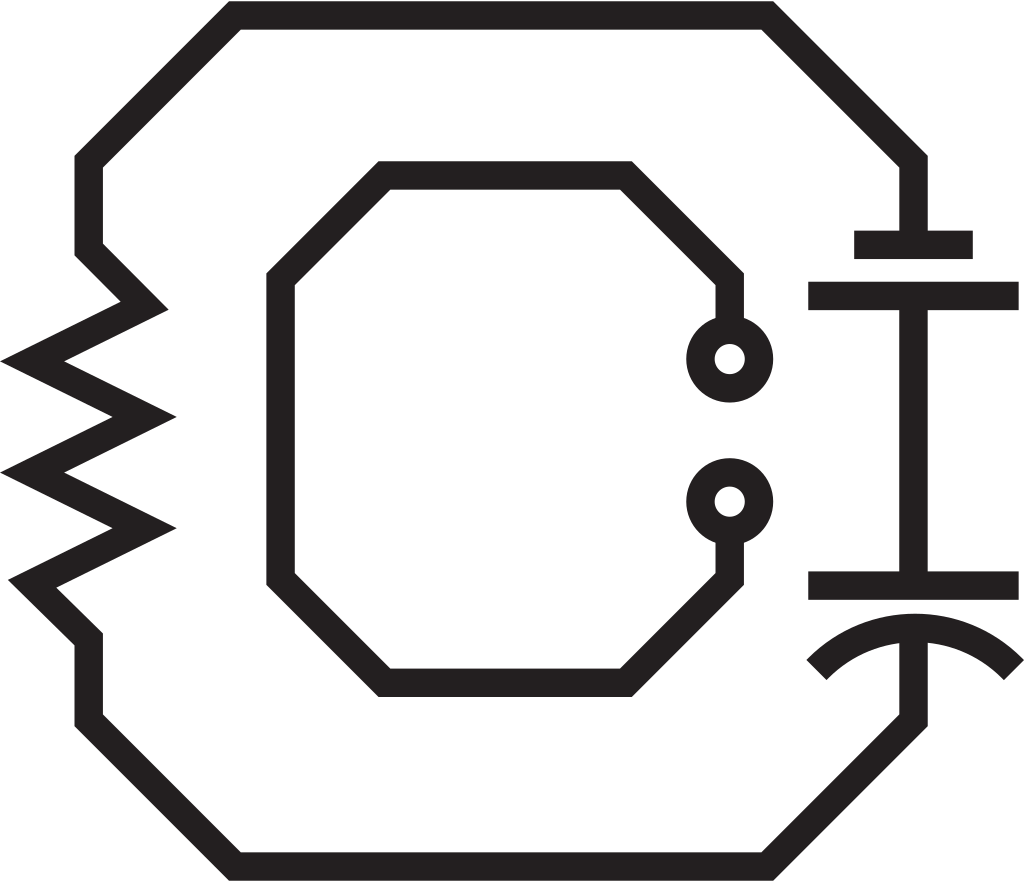
\includegraphics[height=0.635cm]{pictures/logo/c3i.png}%
    \hspace{0.25cm}%
    
\includegraphics[height=0.635cm]{pictures/logo/m1_alpha.pdf}\par
    \vspace{-0.3cm}%
    \textcolor{UDSgreenSolidarite}{%
        \noindent\rule{\textwidth}{1pt}%
    }%
}%

\defbeamertemplate*{footline}{mytheme}{%
    \leavevmode%
    \hbox{%
        \begin{beamercolorbox}%
            [wd=.33\paperwidth, ht=2.25ex, dp=1ex, center]{author in head/foot}%
            \usebeamerfont{author in head/foot}%
                \initials
        \end{beamercolorbox}%
        \begin{beamercolorbox}%
            [wd=.34\paperwidth, ht=2.25ex, dp=1ex, center]%
            {title in head/foot}%
            \usebeamerfont{title in head/foot}%
                \textbf{\inserttitle}%
        \end{beamercolorbox}%
    }%
    \begin{beamercolorbox}%
        [wd=.33\paperwidth, ht=2.25ex, dp=1ex, right]%
        {date in head/foot}%
        \hfill\usebeamerfont{date in head/foot}%
            \today{}%
        \hfill%
        \insertframenumber{} / \inserttotalframenumber%
        \hspace*{2ex}%
    \end{beamercolorbox}%
}%


%!TEX root = ../presentation.tex 


% ---------------------------------------------------------------------------
%  PACKAGES
% ---------------------------------------------------------------------------
\usepackage{tikz}        
\usepackage{etoolbox}     
\usepackage{ifthen}       
% ---------------------------------------------------------------------------
%  GLOBAL DATA
% ---------------------------------------------------------------------------
\newcount\IceSecNum        % counts the *current* section number
\IceSecNum=0               % start at zero

\newcommand{\TotalSecs}{16} % <-- Number of level/section
\newcommand{\IcebergImg}{pictures/iceberg/iceberg-background.png}

% ---------------------------------------------------------------------------
%  TEXT COLOR
% ---------------------------------------------------------------------------
\RequirePackage{xcolor}
\newcommand{\UpdateIcebergTocColor}{%
  \ifnum\IceSecNum<4
      \colorlet{IceFg}{black}% sky & ice
  \else\ifnum\IceSecNum<5
      \colorlet{IceFg}{gray!20!white}% mid‑blue water
  \else
      \colorlet{IceFg}{white}% deep ocean
  \fi\fi
  % apply to all TOC elements we’ll show
  \setbeamercolor{section in toc}{fg=IceFg}%
  \setbeamercolor{subsection in toc}{fg=IceFg}%
  \setbeamercolor{section in toc shaded}{fg=IceFg}%
  \setbeamercolor{subsection in toc shaded}{fg=IceFg}%
}

% ---------------------------------------------------------------------------
%  BACKGROUND TEMPLATE (called for every section title slide)
% ---------------------------------------------------------------------------
\newcommand{\icebergbackground}{%
  % Shift amount = –(section‑1) × (paperheight / TotalSecs)
        \pgfmathsetmacro{\t}{(\IceSecNum-1)/(\TotalSecs-1)}
        \pgfmathsetmacro{\ease}{1/(1+exp(-4*(\t-0.85)))}
        \pgfmathsetmacro{\yShift}{\ease*2872}
  %
  \usebackgroundtemplate{%
    \begin{tikzpicture}[remember picture,overlay]
      \node[anchor=north west, xshift=-10pt] at (current page.north west)
            [yshift=\yShift]  % scroll down as \IceSecNum grows
            {\includegraphics[width=\paperwidth+10pt]{\IcebergImg}};
    \end{tikzpicture}}}

% ---------------------------------------------------------------------------
%  HOOK: increment counter every time \section is called
% ---------------------------------------------------------------------------
\pretocmd{\section}{\global\advance\IceSecNum by 1\relax}{}{}

% ---------------------------------------------------------------------------
%  TOC COLUMN MACRO
% ---------------------------------------------------------------------------


\newcommand{\RightSideTOC}{%
 \UpdateIcebergTocColor
  \begin{columns}[T] % [T] aligns the tops
    \column{.85\textwidth}%
          {\raggedleft
        \tableofcontents[
        sectionstyle=shaded/show,
        subsectionstyle=show/show,
        hideothersubsections,
          sections={
            \number\numexpr\IceSecNum-1\relax,
            \number\IceSecNum,
            \number\numexpr\IceSecNum+1\relax
          }
        ]
        }
    \column{.15\textwidth}%
        %\vfill\centering\maketoctitleheader\vfill

  \end{columns}}






% --------------- BUILD SETTINGS ----------------
\pdfcompresslevel=2
\pdfobjcompresslevel=1


% \tikzexternalize

% \dump
\csname endofdump\endcsname
\endofdump
%mylatex




% ----------------------- BEGIN DOCUMENT ------------------------

\begin{document}

\titlebackground

\begin{frame}[plain]
    \maketitle
\end{frame}

\introbackground

\begin{frame}[plain, label=intro]
    \centering
    \Large

    \textcolor{white}{
        \LARGE{\textbf{\inserttitle}}\\
        \textbf{\textit{\insertsubtitle}}\\
        Par: \insertauthor\\
    }
    \vspace{24pt}
    \begin{tabular}{c l}
        \textcolor{UDSgreenFierte}{\faListOl}
            & \textcolor{white}{~Comment choisir ses composantes et optimiser son BOM?}\\
            [0.3em]
        \textcolor{UDSgreenFierte}{\faMicrochip}
            & \textcolor{white}{~Comment bien conçevoir un symbole et un footprint?}\\
            [0.3em]
        \textcolor{UDSgreenFierte}{\faFirstdraft}
            & \textcolor{white}{~Bonnes pratiques de schémas}\\
            [0.3em]
        \textcolor{UDSgreenFierte}{\faProjectDiagram}
            & \textcolor{white}{~Bonnes pratiques de layout}\\
            [0.3em]
        \textcolor{UDSgreenFierte}{\faClipboardList}
            & \textcolor{white}{~Comment faire un design review?}\\
            [0.3em]
        \textcolor{UDSgreenFierte}{\faComments}
            & \textcolor{white}{~Communication avec fabricants, assembleurs et programmeurs}\\
    \end{tabular}
\end{frame}



% - TOC -
\maketoc

% ------------ SECTIONS -----------

\defaultbackground
%!TEX root = ../presentation.tex 

\section[Level 1]{Surface Ripple [20min]}
\begin{frame}{Introduction}
 Introduction des mathematiques et équation fondamentales à l'electromagnetisme
\end{frame}


\subsection[10min - Max]{EM Fields \rom{1}}
\begin{frame}{Plan}
    \begin{makelist}[\small][1.5]
        \icon{\faCheck} & Champ Vectoriel\\
        \icon[red]{\faTimes} & Divergente, Rotationnelle\\
        \icon[red]{\faTimes} & Regle de la main droite \\
        \icon[red]{\faTimes} & Equation de Maxwell
    \end{makelist}
\end{frame}

\begin{frame}{Champs Vectoriel}
    \begin{twocolumns}[0.4]
        \leftcol
            \makefigure[1.0][0.8][]{level-1/vector-field-1}
        \rightcol
           \makefigure[1.0][0.8][]{level-1/vector-field-2}
    \end{twocolumns}
\end{frame}

\begin{frame}{Champs Vectoriel}
    \centering
    Le champs électromagnétiques sont "encodé" dans 2 champs. \\
    Par contre, les équations utilisent 4 champs vectoriels pour les représenter\\
    \vspace{15pt}
    \begin{twocolumns}[0.4]
        \leftcol
            \centering
            \underline{Intensitée du Champ Électrique}
            \begin{equation*}
                \efield \rightarrow [\SI{}{\volt\per\meter}]
            \end{equation*}
            \underline{Densitée de Flux Électrique}
            \begin{equation*}
                \eflux \rightarrow [\SI{}{\coulomb\per\meter\squared}]
            \end{equation*}
            \underline{Relation}
            \begin{equation*}
                \eflux = \varepsilon \efield
            \end{equation*}
        \rightcol
            \centering
            \underline{Intensitée de Champ Magnétique}
            \begin{equation*}
                \mfield \rightarrow [\SI{}{\ampere\per\meter}]
            \end{equation*}
            \underline{Densitée de Flux Magnétique}
            \begin{equation*}
                \mflux \rightarrow [\SI{}{\weber\per\meter\squared} \;\; ou \;\; \SI{}{\tesla}]
            \end{equation*}
            \underline{Relation}
            \begin{equation*}
                \mflux = \mu \mfield
            \end{equation*}
    \end{twocolumns}
\end{frame}

\begin{frame}{Dérivée Temporelle vs. Spatiale}
    \centering
    On peut décrire le comportement de ces champs en utilisant\\
    le calcul vectoriel:
    \vspace{15pt}
    \begin{twocolumns}[0.5]
        \leftcol
            Dérivée Temporelle
        \rightcol
           Dérivée Spatiale:
            \begin{equation}
                \text{Divergence} = \nabv \cdot \vec{V}
            \end{equation}
            \begin{equation}
                \text{Curl} = \nabv \times \vec{V}
            \end{equation}
    \end{twocolumns}
\end{frame}

\begin{frame}{Divergence}
    \begin{equation}
        \nabv \cdot \vec{V} = \frac{\partial \vec{V_x}}{\partial x} + \frac{\partial \vec{V_y}}{\partial y} + \frac{\partial \vec{V_z}}{\partial z}
    \end{equation}
    \makefigure[1.0][0.6][]{level-1/divergence}
\end{frame}

\begin{frame}{Gauss's Law}
    \begin{twocolumns}[0.5]
    \leftcol
        \centering{\underline{Gauss's Law}}
        \vspace{-8pt}
        \begin{equation}
            \nabv \cdot \efield = \frac{\rho}{\varepsilon_0}
            \hspace{1em} \Longleftrightarrow \hspace{1.0em}
            \nabv \cdot \eflux = \rho v
        \end{equation}
    \rightcol
        \makefigure[1.0][0.5][]{level-1/gauss-law-1}
    \end{twocolumns}
\end{frame}
 
\begin{frame}{E Field on a PCB}
    \vspace{-20pt}
    \makefigure[1.0][1.0][]{level-1/pcb-E-fields-before}
\end{frame}

\begin{frame}{E Field on a PCB}
    \vspace{-20pt}
    \makefigure[1.0][1.0][]{level-1/pcb-E-fields}
\end{frame}

\begin{frame}{Gauss's Law for Magnetism}
    \begin{twocolumns}[0.35]
        \leftcol
            \centering{\underline{Gauss's Law For Magnetism}}
            \vspace{-8pt}
            \begin{equation}
                \nabv \cdot \mflux = 0
            \end{equation}
        \rightcol
            \makefigure[1.0][0.75][]{level-1/magnets}
    \end{twocolumns}
\end{frame}

\begin{frame}{Gauss's Law for Magnetism}
    \begin{twocolumns}[0.35]
        \leftcol
            \centering{\underline{Gauss's Law For Magnetism}}
            \vspace{-8pt}
            \begin{equation}
                \nabv \cdot \mflux = 0
            \end{equation}\\
            \vspace{10pt}
            \makefigure[1.0][0.4][]{level-1/magnetic-meme}
        \rightcol
            \makefigure[1.0][0.5][]{level-1/magnetic-meme-2}
    \end{twocolumns}
\end{frame}



\begin{frame}{Curl}
    \begin{equation}
        \nabv \times \vec{V} = \left(\frac{\partial\vec{V_z}}{\partial y}-\frac{\partial\vec{V_y}}{\partial z} \right) \check{x} +
        \left(\frac{\partial\vec{V_x}}{\partial z}-\frac{\partial\vec{V_z}}{\partial x} \right) \check{y} +
        \left(\frac{\partial\vec{V_y}}{\partial x}-\frac{\partial\vec{V_x}}{\partial y} \right) \check{z}
    \end{equation}

\begin{twocolumns}[0.5]
    \leftcol
        \makefigure[1.0][0.5][]{level-1/cyclone}
    \rightcol
        \makefigure[1.0][0.5][]{level-1/curl-ball}
 \end{twocolumns}
\end{frame}

\begin{frame}{Curl}
    \begin{makelist}[\small][1.5]
        \icon[red]{\faExclamationTriangle} & \textbf{ATTENTION:} La Rotationnelle n'a pas de définition en 2D! Il faut au moin 3 dimensions!
    \end{makelist}
\end{frame}

\begin{frame}{Faraday's Law of Induction}
    \begin{twocolumns}[0.35]
    \leftcol
        \centering{\underline{Faraday's Law of Induction}}
        \vspace{-10pt}
        \begin{equation}
            \nabv \times \efield = -\ddt{\mflux}
        \end{equation}
    \rightcol
        \makefigure[1.0][0.8][]{level-1/generator}
 \end{twocolumns}

\end{frame}

\begin{frame}{Ampère-Maxwell's Law}
    \centering{\underline{Ampère-Maxwell's Law}}
    \vspace{-10pt}
    \begin{equation}
        \nabv \times \mfield = \ddt{\eflux} + \ecurrent
        \hspace{1em} \Longleftrightarrow \hspace{1.0em}
        \nabv \times \mflux = \mu_0 \varepsilon_0 \ddt{\efield} + \mu_0 \ecurrent
    \end{equation}
\end{frame}

\begin{frame}{E Field on a PCB}
    \vspace{-20pt}
    \makefigure[1.0][1.0][]{level-1/pcb-H-fields-before}
\end{frame}

\begin{frame}{E Field on a PCB}
    \vspace{-20pt}
    \makefigure[1.0][1.0][]{level-1/pcb-H-fields}
\end{frame}

\begin{frame}{Maxwell Equation}
    \begin{twocolumns}[0.3]
    \leftcol
        \makefigure[1.0][0.8][James Clark Maxwell]{level-1/james-maxwell}
    \rightcol
        \centering{\underline{Gauss's Law}}
        \vspace{-8pt}
        \begin{equation}
                \nabv \cdot \efield = \frac{\rho}{\varepsilon_0}
                \hspace{1em} \Longleftrightarrow \hspace{1.0em}
                \nabv \cdot \eflux = \rho v
        \end{equation}
        \centering{\underline{Gauss's Law For Magnetism}}
        \vspace{-8pt}
        \begin{equation}
            \nabv \cdot \mflux = 0
        \end{equation}
        \centering{\underline{Faraday's Law of Induction}}
        \vspace{-10pt}
        \begin{equation}
            \nabv \times \efield = -\ddt{\mflux}
        \end{equation}
        \centering{\underline{Ampère-Maxwell's Law}}
        \vspace{-10pt}
        \begin{equation}
            \nabv \times \mfield = \ddt{\eflux} + \ecurrent
            \hspace{1em} \Longleftrightarrow \hspace{1.0em}
            \nabv \times \mflux = \mu_0 \varepsilon_0 \ddt{\efield} + \mu_0 \ecurrent
        \end{equation}
 \end{twocolumns}
\end{frame}

\begin{frame}{EM Field on a PCB}
    \vspace{-20pt}
    \makefigure[1.0][1.0][]{level-1/pcb-fields}
\end{frame}

\subsection[1min - Max]{Superposition \rom{1}}

\begin{frame}{Équations linéaires}
    Équation linéaire:
    \begin{equation}
        y = mx+b
    \end{equation}
    Équation non-linéaire:
    \begin{equation}
        y = ax^2 + mx + b
    \end{equation}
\end{frame}

\begin{frame}{Principe}
    Les Équations de Maxwell sont \textbf{linéaires} cela veux dire qu'on peut utiliser le \textbf{Principe de Superposition}\\
    \vspace{20pt}
    Cela veut dire que la sortie d'un système avec plusieurs stimulis en entrée, sera \textbf{la somme} de tout les stimulis en sortie.\\
    \vspace{20pt}
    \begin{equation}
        V_{out} = \sum v_{out}
    \end{equation}
\end{frame}

\begin{frame}{Green Theorem}
    \begin{twocolumns}[0.5]
        \leftcol
            \makefigure[1.0][0.7][]{level-1/green-theorem-meme}
        \rightcol
            \makefigure[1.0][0.7][Inductor Magnetic field]{level-1/inductor-magnetic-field}
    \end{twocolumns}
\end{frame}

\subsection[2min - Max]{Voltage}
\begin{frame}{Plan}
    \begin{twocolumns}[0.5]
        \leftcol
            \begin{center}
            Energie Potentielle Gravitationnelle [J]:
            \end{center}
        \rightcol
            \begin{center}
            Potentiel Électrique [J/C]:\\
            \end{center}
    \end{twocolumns}
    \begin{twocolumns}[0.5]
        \leftcol
            \begin{equation}
                U_{g} = \int_{A}^{B}\vec{F_g} \,dl =  mgh
            \end{equation}
        \rightcol
            \begin{equation}
                \Delta V_{AB} = -\int_{A}^{B}\efield \,dl
            \end{equation}
    \end{twocolumns}
    \vspace{-24pt}
    \begin{twocolumns}[0.5]
        \leftcol
            \makefigure[1][0.75][]{level-1/gravitationnal-potential}
        \rightcol
            \makefigure[1][0.5][]{level-1/voltage}
    \end{twocolumns}
    \vfill
\end{frame}

\subsection[2min - Max]{Courant}
\begin{frame}{Plan}
    \begin{equation}
        \Icurrent = \iint_A \ecurrent \,dA
    \end{equation}\\
    \vspace{20pt}
    \makefigure[0.8][0.8][\textcolor{red}{Might change for my own image later}]{level-1/current-density}
\end{frame}


\begin{frame}{Mouvement de Charges}
    \centering
    \icon[green]{\faExclamationTriangle} \textbf{ATTENTION:} Le courant $\Icurrent$ montre le sens des \textbf{Charges Positives}!\\
    Les électrons vont dans le \textbf{sens contraire}!\\
    \vspace{20pt}
    \textcolor{red}{Sa serait cool d'avoir un de tes Tikz de circuit pour montrer la difference entre electron et courant conventionnel}
\end{frame}

\begin{frame}{Conductivitée}
    \centering
    \icon[green]{\faExchange*} Represente la capacité d'un matériaux à conduire un courant électrique.\\
    Plus la conductivitée est haute, plus il est facile pour les électrons de circuler.\\
    \vspace{30pt}
    La conductivitée \textbf{$\sigma$} est l'inverse de la resistivité \textbf{$\rho$}:
    \begin{equation}
        \sigma = \frac{1}{\rho} \hspace{2.0em} [\Omega^{-1} m^{-1} \;\;\text{ou}\;\; S\cdot m^{-1}]
    \end{equation}
\end{frame}

\begin{frame}{Conductivitée}
    \centering
    \icon[red]{\faThermometerThreeQuarters} Il y a une relation interessante entre la conductivité thermique et électrique.
    \makefigure[0.6][0.7][]{level-1/conductivity-graph}
\end{frame}

\begin{frame}{Conductivitée selon température}
\end{frame}

\subsection[1min - Max]{Lois d'Ohm}
\begin{frame}{Ohm's Law in Vector form}
        \begin{twocolumns}[0.5]
        \leftcol
        \begin{equation}
            \ecurrent = \sigma \efield
        \end{equation}
        \rightcol
        \makefigure[1.0][1.0][]{level-1/pcb-fields}
    \end{twocolumns}        
\end{frame}

\begin{frame}{Comparaison}
        \begin{twocolumns}[0.5]
        \leftcol
            \centering
            \underline{Vue Schematique:}
            \begin{equation*}
                V = R I
            \end{equation*}
        \rightcol
            \centering
            \underline{Vue Layout:}
            \begin{equation*}
                \ecurrent = \sigma \efield
            \end{equation*}
    \end{twocolumns}
    \vspace{30pt}
    \centering
    Nous allons voir plus loin pourquoi il est important\\ de considérer la forme vectorielle de la loi d'Ohm en layout
\end{frame}

\subsection[2min - Max]{Matériaux \rom{1}}
\begin{frame}{Plan}
    \begin{makelist}[\small][1.5]
        \icon[red]{\faTimes} & Retour sur $\mu$ \& $\varepsilon$\\
        \icon[red]{\faTimes} & Difference entre $\varepsilon$, $\varepsilon_0$ et $\varepsilon_r$\\
        \icon[red]{\faTimes} & Indices de refraction Reel
    \end{makelist}
\end{frame}

\begin{frame}{Permittivitée vs. Permeabilitée}
    \begin{twocolumns}[0.5]
        \leftcol
            Permittivity
        \rightcol
            Permeability
    \end{twocolumns}
\end{frame}

\begin{frame}{$\varepsilon$ \& $\mu$}
    \begin{twocolumns}[0.5]
        \leftcol
            \begin{equation}
                \varepsilon = \text{Electric Permittivity [F/m]}
            \end{equation}
            \begin{equation}
                \mu = \text{Magnetic Permeabililty [H/m]}
            \end{equation}
        \rightcol
            \makefigure[1.0][0.7][Imperméable]{level-1/impermeable}
    \end{twocolumns}
\end{frame}

\begin{frame}{$\varepsilon_0$ \& $\mu_0$}
    \begin{twocolumns}[0.5]
        \leftcol
            Electric Free Space Permittivity [F/m]:
            \begin{equation}
                \varepsilon_0 \approx 8.854\times 10^{-12}
            \end{equation}
            Magnetic Free Space Permeabililty [H/m]:
            \begin{equation}
                \mu_0 \approx 4\pi \times 10^{-7}
            \end{equation}
        \rightcol
            \makefigure[1.0][0.7][Imperméable]{level-1/impermeable}
    \end{twocolumns}
\end{frame}

\begin{frame}{$\varepsilon_r$ \& $\mu_r$}
    \begin{twocolumns}[0.5]
        \leftcol
            Electric Relative Permittivity [F/m]:
            \begin{equation}
                \varepsilon_r =\frac{\varepsilon}{\varepsilon_0}
            \end{equation}
            Magnetic Relative Permeabililty [H/m]:
            \begin{equation}
                \mu_r =\frac{\mu}{\mu_0}
            \end{equation}
        \rightcol
            \makefigure[1.0][0.7][Imperméable]{level-1/impermeable}
    \end{twocolumns}
\end{frame}

\begin{frame}{Indice de Refraction}
    \begin{twocolumns}[0.5]
        \leftcol
            Indice de refraction pour materiaux \textbf{sans pertes}:
            \begin{equation}
                n =\frac{\sqrt{\varepsilon \mu}}{\sqrt{\varepsilon_0 \mu_0}} = \sqrt{\varepsilon_r \mu_r}
            \end{equation}
        \rightcol
            \makefigure[1.0][0.7][Radio Telescope]{level-1/rf-telescope}
    \end{twocolumns}
\end{frame}


\begin{comment}
\subsection[4min - Max]{Charge Movement}
\begin{frame}{Plan}
    \begin{makelist}[\small][1.5]
        \icon[red]{\faTimes} & Comment les Electrons bougent\\
        \icon[red]{\faTimes} & Propriété materiaux
    \end{makelist}
\end{frame}

\begin{frame}{EM Properties of metals}
    \maketable{conductivity}
\end{frame}


\subsection[3min - Max]{Passive Components \rom{1}}
\begin{frame}{Plan}
    \begin{makelist}[\small][1.5]
        \icon[red]{\faTimes} & Resistance\\
        \icon[red]{\faTimes} & Condensateur \\
        \icon[red]{\faTimes} & Inducteur
    \end{makelist}
\end{frame}
\end{comment}
%!TEX root = ../presentation.tex

\section[Level 2]{Current Paths [30min-50min]}


\subsection[2min-Pascal]{Signal Source \rom{1}}
\begin{frame}{Comparaison des sources}
    \begin{twocolumns}
        \leftcol
        \begin{center}
            \textbf{Source de tension}
        \end{center}
        \rightcol
        \begin{center}
            \textbf{Source de courant}
        \end{center}
    \end{twocolumns}

    \begin{twocolumns}[0.55]
        \leftcol
        \begin{itemize}
            \item Modèle plus traditionnel
            \item Fournit une tension fixe peu importe le courant demandé
            \item Tension cause un courant au travers d'une load
        \end{itemize}

        \rightcol
        \begin{itemize}
            \item Fournit un courant fixe peu importe la tension requise pour driver ce courant demandé
            \item Courant au travers d'une load crée une tension
        \end{itemize}
        
    \end{twocolumns}

    \vspace{-8pt}
    \begin{twocolumns}
        \leftcol
        \begin{center}
            $I = \dfrac{V}{R}$
        \end{center}
        \rightcol
        \begin{center}
            $V = RI$
        \end{center}
    \end{twocolumns}

    \vfill

    \begin{twocolumns}
        \leftcol
        \begin{maketikzfigure}[1][0.25]
            \draw (0, 0) node[ground]{}
                to [V, l=$V_S$, invert] ++(0, 2.5)
                to [short] ++(2.5, 0)
                to [R, l_=$R_{LOAD}$,i={$I = \frac{V_S}{R_{LOAD}}$}] ++(0, -2.5)
                to node[ground]{} ++(0, 0);
        \end{maketikzfigure}
        \rightcol
        \begin{maketikzfigure}[1][0.25]
            \draw (0, 0) node[ground]{}
                to [I, l=$I_S$] ++(0, 2.5)
                to [short, i=$I_S$] ++(2.5, 0)
                to [R, l_=$R_{LOAD}$,v^={$V = I_S \cdot R_{LOAD}$}] ++(0, -2.5)
                to node[ground]{} ++(0, 0);
        \end{maketikzfigure}
    \end{twocolumns}
\end{frame}

\begin{frame}{Exemples de sources}
    \begin{itemize}
    \only<1->{
        \item[] \itemicon{\faBatteryThreeQuarters} \textbf{Batteries}
        \begin{itemize}
            \item[] Réaction chimique qui fournit un potentiel de tension fixe aux bornes de la cellule.
        \end{itemize}
    }
    \only<2->{
        \item[] \itemicon{\faSun} \textbf{Effect Photovoltaïque}

        \begin{itemize}
            \item[] Excitation d'électrons frappés par des photons dans un matériau semiconducteur, causant leur déplacement.
        \end{itemize}
    }
    \only<3->{
        \item[] \itemicon{\faThermometerHalf} \textbf{Effect Seebeck}
        \begin{itemize}
            \item[] Effet thermoélectrique qui produit un différentiel de tension entre deux métaux différents qui ont des énergies thermiques différentes.
        \end{itemize}
    }
    \only<4->{
        \item[] \itemicon{\faVolumeUp} \textbf{Effect Piézoélectrique}
        \begin{itemize}
            \item[] Charge électrique provenant d'un matériau dont la matrice crystalline est déformée mécaniquementé.
        \end{itemize}
    }
    \only<5->{
        \item[] \itemicon{\faBolt} \textbf{Transistor Bipolaire --- Miroir de Courant}
        \begin{itemize}
            \item[] Deux effets qui répliquent un courant (avec un multiplicateur) en utilisant des transistors.
        \end{itemize}
    }
    \only<5->{
        \item[] \itemicon{\faSync} \textbf{Induction Électromagnétique}
        \begin{itemize}
            \item[] Le sujet de cette présentation.
        \end{itemize}
    }
    \end{itemize}
\end{frame}

\begin{frame}{Sources dans la vraie vie}
    \begin{itemize}
        \item Une vraie source de courant n'existe pas
        \item Une vraie source de tension n'existe pas
        \bigskip
        \item Tout ce qui existe sont des sources de puissances
        \item Les "sources" utilisent du feedback pour réguler courant et/ou tension
        \bigskip
        \item Il existe des sources de résistance aussi
    \end{itemize}
\end{frame}

\subsection[3min - Max]{Harmonics \rom{1}}
\begin{frame}{Plan}
    \begin{makelist}[\small][1.5]
        \icon[red]{\faTimes} & Transformé de fourier\\
        \icon[red]{\faTimes} & Addition de Signaux \\
        \icon[red]{\faTimes} & Taylor \\
        \icon[red]{\faTimes} & Harmonique paires/impaires
    \end{makelist}
\end{frame}

\begin{frame}{Square Wave}
    \makefigure[1.0][0.7][]{level-2/harmonic-meme}
\end{frame}

\subsection[5min-Pascal]{Propagation Speed \rom{1}}
\begin{frame}{Plan}
    \begin{makelist}[\small][1.5]
        \icon[red]{\faTimes} & Vitesse de propagation\\
        \icon[red]{\faTimes} & Velocite de phase ($n=\frac{c}{v_p}$)\\
        \icon[red]{\faTimes} & Speed of light\\
    \end{makelist}
\end{frame}

\begin{frame}{Phase Velocity}
    \maketable{phase-velocity}
\end{frame}


\subsection[5min-Pascal]{Ground planes \rom{1}}
\begin{frame}{Plan}
    \begin{makelist}[\small][1.5]
        \icon[red]{\faTimes} & Item 1\\
        \icon[red]{\faTimes} & Item 2\\
        \icon[red]{\faTimes} & GND IS NOT A SINK, IT'S A REFERENCE
    \end{makelist}
    
\end{frame}

\subsection[5min-Pascal/Max]{Induction}
\begin{frame}{Plan}
    \begin{makelist}[\small][1.5]
        \icon[red]{\faTimes} & Comment les courants sont induits \\
        \icon[red]{\faTimes} & Regle de la main droite\\
        \icon[red]{\faTimes} & Item 3
    \end{makelist}
\end{frame}

\subsection[5min-Pascal]{Current loops}
\begin{frame}{Plan}
    %Perso je splitterais cette section en 2 avec une partie plus deep dans l'iceberg
    \begin{makelist}[\small][1.5]
        \icon[red]{\faTimes} & GND Loop avec cable(Ou on place ca apres la section noise?)\\
        \icon[red]{\faTimes} & Frequency dependant loop\\
        \icon[red]{\faTimes} & Item 3
    \end{makelist}
\end{frame}

\begin{frame}{Quote}
    \begin{makelist}[\small][1.5]
        \icon[red]{\faTimes} & L'Électricité prend le chemin le plus court\\
        \icon[green]{\faCheck} & L'Électricité prend le chemin avec la plus petite Resistance\\ 
    \end{makelist}
\end{frame}

\subsection[3min-Max]{Radiation \rom{1}}
\begin{frame}{Plan}
    \begin{makelist}[\small][1.5]
        \icon[red]{\faTimes} & Inductor field\\
        \icon[red]{\faTimes} & Sun Coronal Mass ejection Analogy\\
        \icon[red]{\faTimes} & Simple Travelling wave\\
        \icon[red]{\faTimes} & Wavelength\\
        \icon[red]{\faTimes} & Induction is actually radiation
    \end{makelist}
\end{frame}

\begin{frame}{Let's talk about Auroras}
\begin{twocolumns}[0.3]
    \leftcol
        \makefigure[1.0][0.7][Auroras]{level-2/auroras}
    \rightcol
        \makefigure[1.0][0.7][Sun Flare]{level-2/CME-blast}
    \end{twocolumns}
\end{frame}

\begin{frame}{Coronal Mass Ejection}
    \begin{twocolumns}[0.5]
        \leftcol
            \makefigure[1.0][0.7][Auroras]{level-2/coronal-mass-ejection}
        \rightcol
            \makefigure[1.0][0.7][Sun Flare]{level-2/coronal-mass-ejection-step}
    \end{twocolumns}
\end{frame}

\begin{frame}{How it relates to an Inductor}
    \begin{twocolumns}[0.5]
        \leftcol
            \makefigure[1.0][0.7][Inductor]{level-1/inductor}
        \rightcol
            \makefigure[1.0][0.7][Inductor Magnetic field]{level-1/inductor-magnetic-field}
    \end{twocolumns}
\end{frame}

\begin{frame}
    \begin{twocolumns}[0.5]
        \leftcol
            \makefigure[1.0][0.7][Magnetic field loop]{level-2/coronal-mass-ejection-loop}
        \rightcol
            \makefigure[1.0][0.7][Inductor Magnetic field]{level-1/inductor-magnetic-field}
    \end{twocolumns}
\end{frame}

\begin{frame}
    \begin{twocolumns}[0.5]
        \leftcol
            \makefigure[1.0][0.7][Magnetic Field Ejection]{level-2/coronal-mass-ejection-step}
        \rightcol
            \makefigure[1.0][0.7][Inductor Magnetic field]{level-1/inductor-current}
    \end{twocolumns}
\end{frame}

\subsection[5min-Pascal]{Fil d'une année lumière de long }
% Parasitiques
\begin{frame}{Plan}
    \begin{makelist}[\small][1.5]
        \icon[red]{\faTimes} & Item 1\\
        \icon[red]{\faTimes} & Item 2\\
        \icon[red]{\faTimes} & Item 3
    \end{makelist}
\end{frame}
%!TEX root = ../main.tex 

\section{Bonnes pratiques de schéma}

\subsection{Clareté}
% Éviter tous les croisements, pas de GND dans les airs, aligner
% Utiliser la grille
% Utiliser des net names
% Quand utiliser des net locaux, globaux, power
% Inputs à gauche, output à droite
% Garder les sections modulaires, bien indiquer les sections, prend de l'espace
% Tout devrait être dans le schematics
%  - Mettre plus que pas assez
%  - Notes pour le programmeur, pour le layouteur, pour l'assembleur
%  - Tu ne devrais pas avoir à réouvrir une datasheet
% Mettre des couleurs sur les nets
% Utiliser des net classes
% Éviter les longues traces qui passent au travers du schéma
% Regrouper des nets en bus

\subsection{Notes}
% Mettre un schéma-bloc et un arbre d'alimentation
%     Draw.io
%     Travailler en hiérarchique
% Calculer le power pour chaque bloc et page
% Mettre des notes avec tous les calculs
% Mettre des notes avec pages de datasheets
% Mettre les courbes d'efficacité etc.
% Cartouche
% Indiquer les tailles et tolérances de composantes sur le schematic
% Notes pour les pins
% - Qu'est-ce qu'elles font, comment configurer
% Essayer le plus possible de garder tout le texte horizontal

\subsection{Testpoints et Debugging}
% Valider les boot sequences & power-sequence
% Se servir des pins flottantes
%  - Ajouter IO, LED, Testpoint, UART
% Mettre des systèmes de mesure de courant
% Met toujours plus de testpoints qu'on pense
%  - Différents types de testpoints

\subsection{Outils}
% Les 0R sont tes amis
%  - Peut remplacer une ferrite ou une shunt
%  - Pins EN et CFG
%  - Solder Bridge Pads
% Pull-ups / Pull-downs pour des pins de configuration
% Utiliser plusieurs pages / Faire un schéma hiérarchique
% Utiliser les Net Classes

\subsection{Autre}
% Toujours mettre des protections
%  - ESD
%  - Power
% Une connection I2C inter-board; mettre des pull-ups sur les deux boards
% Export ton schematic en PDF pour l'ouvrir sans logiciel
% 0.1µF

\subsection{Design Review}
% Faire réviser par quelqu'un d'autre après
% Passer le DRC / ERC
% Pour chaque composante:
%  - Valider le footprint
%  - Valider le symbole
%    - Numéros de pins selon la pièce choisie dans le BOM
%  - Valider chacune des connections en retournant vérifier dans la datasheet
%    - Est-ce que je suis au bon niveau de tension?
%    - Est-ce que j'ai besoin de pull-ups / pull-downs / autres passives
%  - Valider le découplage selon les fréquences
%  - Est-ce que le schéma est facilement lisible?
% Faire une review du BOM
%  - Est-ce que j'ai des erreurs de copier-coller?
%  - Est-ce que j'ai le bon modèle de pièce dans le BOM?
%    - Version SOIC vs version QFN
%    - Version pour un autre niveau de tension
%    - Version qui vient dans un paquet de 1000 au minimum
%  - Est-ce que j'ai toutes mes pièces mécaniques dans le BOM (standoffs, vis, washer, nut, heatsinks)
% Valider le debugging
%  - Est-ce que j'ai assez de testpoints (+ de GND!)
%  - Est-ce que j'ai des ports de debug sur mon MCU/FPGA
%  - Est-ce que j'ai des 0R pour ma configuration?
% Revalider tous les calculs
%  - Trucs changent pendant le design et ne sont pas toujours mis à jour
%  - Diviseurs de tension
%  - Dimentionnement des pièces

%%!TEX root = ../presentation.tex

\section{Level 5: Crosstalk \& Coupling [18min - 1h55]}

\subsection{Radiation II [3min - Max]}
% Radiation Pattern

\subsection{Differential Pairs [5min - Pascal]}
% Do Differential Pairs need GND?

\subsection{Far crosstalk [5min - Pascal]}

\subsection{Near crosstalk [5min - Pascal]}

%%!TEX root = ../presentation.tex
\pascalbackground

\begin{frame}{Comment fonctionne un crystal}
    \begin{twocolumns}[0.66]
        \leftcol
            \begin{itemize}
                \item Oscillateur utilisant l'effet piézoélectrique
                \item Déformation mécanique d'une matrice cristalline
                \item Génère un champ électrique
                \item Effet inverse possible!
                \bigskip
                \item Fréquence de résonance
                \item Q factor beaucoup plus élevé que circuit RLC équivalent
            \end{itemize}
        \makefigure[1][0.35]{level-5/piezoelectric-effect}
        \rightcol
            \begin{maketikzfigure}[1][0.66]
                \draw (0, 6) node[vcc] {};
                \draw (0, 6) to [short] (-1, 6) to 
                [R, l=$R_1$] (-1, 4) to
                [american inductor, l=$L_1$] (-1, 2) to
                [C, l=$C_1$] (-1, 0) to
                [short] (0, 0) 
                node[ground] {};

                \draw (0, 6) to [short] (1, 6) to
                [C, l=$C_2$] (1, 0) to 
                [short] (0, 0);
            \end{maketikzfigure}
    \end{twocolumns}
\end{frame}

\begin{frame}{Comment résonne un crystal}
    \begin{twocolumns}[0.33]
        \leftcol
            \begin{maketikzfigure}
                \draw (0, 6) node[vcc] {};
                \draw (0, 6) to [short] (-1, 6) to 
                [R, l=$R_1$, color=UDSviolet] (-1, 4) to
                [american inductor, l=$L_1$, color=orange] (-1, 2) to
                [C, l=$C_1$, color=blue] (-1, 0) to
                [short] (0, 0) 
                node[ground] {};

                \draw (0, 6) to [short] (1, 6) to
                [C, l=$C_2$, color=red] (1, 0) to 
                [short] (0, 0);
            \end{maketikzfigure}
        \rightcol

            \begin{maketikzfigure}
            \begin{axis}[
              width=12cm, height=6.5cm,
              axis lines=left,
              xlabel={$f$}, ylabel={$Z$},
              xmin=0, xmax=1, ymin=0, ymax=1,
              xtick=\empty, ytick=\empty,
              clip=false
            ]

            \addplot[ultra thick, accent, smooth]
              coordinates {
                (0.02, 0.92) (0.10, 0.60) (0.22, 0.22)             % falling, capacitive
                (0.30, 0.30) (0.38, 0.55) (0.46, 0.80)             % rising to parallel resonance
                (0.52, 0.88) (0.62, 0.62) (0.78, 0.48) (0.98,0.36) % roll-off
              };

            \def\xFs{0.26}
            \def\xFr{0.50}

            \draw[dashed] (axis cs:\xFs,0) -- (axis cs:\xFs, 1);
            \draw[dashed] (axis cs:\xFr,0) -- (axis cs:\xFr, 1);

            \draw[color=UDSviolet, thick] (axis cs:0, 0.20) -- (axis cs:1, 0.20);

            \node[above] at (axis cs:\xFs, 1) {$f_s$};
            \node[above] at (axis cs:\xFr, 1) {$f_r$};

            \node[anchor=south west] at (axis cs:0.02, 1) {\small Capacitif};
            \node[anchor=south]      at (axis cs:0.38, 1) {\small Inductif};
            \node[anchor=south east] at (axis cs:0.98, 1) {\small Capacitif};

            \node[below] at (axis cs:\xFs,0) {\scriptsize Résonance Série};
            \node[below] at (axis cs:\xFr,-0.1) {\scriptsize Résonance Parallèle};

            \end{axis}
                
            \end{maketikzfigure}
    \end{twocolumns}
\end{frame}

\begin{frame}{Crystal sur un microcontrôleur}
    \ctikzset{bipoles/capacitor/height=0.5}
    \ctikzset{bipoles/capacitor/width=0.2}
    \ctikzset{logic ports/scale=0.5}
    \begin{maketikzfigure}

        \draw (4, 0) node [dipchip,
            num pins = 8,
            hide numbers,
            external pins width=0.3,
            external pad fraction=4,
            ](IC){};

            \node [right, font=\tiny] at (IC.bpin 1) {OSC2};
            \node [right, font=\tiny] at (IC.bpin 4) {OSC1};


            \draw[thick] (IC.pin 1) to [short] ($(IC.pin 1) - (1.5, 0)$) to
            [piezoelectric, color=accent] ($(IC.pin 4) - (1.5, 0)$) to
            [short] (IC.pin 4);

            \only<1, 3>{
                \draw[thick] ($(IC.pin 1) - (1.5, 0)$) to
                [C, l=$C_1$] ($(IC.pin 1) - (3.5, 0)$);
                \draw[thick] ($(IC.pin 4) - (1.5, 0)$) to
                [C, l=$C_2$] ($(IC.pin 4) - (3.5, 0)$);
            }
            \only<2, 4->{
                \draw[thick] ($(IC.pin 1) - (1.5, 0)$) to
                [C, l=$C_1$, color=accent2] ($(IC.pin 1) - (3.5, 0)$);
                \draw[thick] ($(IC.pin 4) - (1.5, 0)$) to
                [C, l=$C_2$, color=accent2] ($(IC.pin 4) - (3.5, 0)$);
            } 

            \draw[thick] ($(IC.pin 1) - (3.5, 0)$) to [short] ($(IC.pin 4) - (3.5, 0)$)
            to [short]   ($(IC.pin 4) - (3.5, 1)$) node[ground]{};


            \only<3->{
                \draw[dashed] (IC.bpin 1) to [short] ($(IC.pin 1) + (1.5, 0)$) to [open]
                ($(IC.pin 4) + (1.5, 0)$) to [short] (IC.bpin 4);

                \draw ($(IC.pin 1) + (1.5, 0)$) to [inline not, color=accent2] ($(IC.pin 4) + (1.5, 0)$);
            }

            \only<4->{
                \draw[->, color = accent]    ($(IC.pin 1) + (2, 0)$)    -- ($(IC.pin 4) + (2, 0)$)    node[midway, below, sloped] {$+\ang{180}$};
                \draw[<-, color = UDSviolet] ($(IC.pin 1) - (0.75, 0)$) -- ($(IC.pin 4) - (0.75, 0)$) node[midway, below, sloped] {$+\ang{180}$};
            }
    \end{maketikzfigure}
\end{frame}

\begin{frame}{Condensateur de charge}
    \begin{twocolumns}
        \leftcol
        \only<1>{
        \begin{itemize}
            \item Les circuits de lecture CMOS d'oscillateur rajoutent une phase de $\ang{180}$
            \item Phase doit être compensée pour atteindre $\ang{360}$
            \item Condensateurs viennent compléter le modèle RLCC du crystal
            \item Crystaux calibrés pour des valeurs de condensateurs $C_L$
        \end{itemize}
        }

        \only<2->{
            \begin{tabular}{l | c}
                \multicolumn{2}{c}{\textbf{\textbf{ESC-16-20S-4X}}}\\
                \hline
                \textbf{Frequency}             & $\SI{16}{\mega\hertz}$\\
                \textbf{Frequency Tolerance}   & $\pm 30\,ppm$\\
                \textbf{Frequency Stability}   & $\pm 50\,ppm$\\
                \textbf{Shunt Capacitance}     & $\SI{7}{\pico\farad}$\\
                \textbf{Load Capacitance}      & $\SI{20}{\pico\farad}$\\
                \textbf{Operating Temperature} & $\SI{-10}{\celsius} à \SI{70}{\celsius}$\\
                \textbf{Storage Temperature}   & $\SI{-55}{\celsius} à \SI{125}{\celsius}$\\
                \textbf{ESR Max}               & $\SI{40}{\ohm}$\\
            \end{tabular}
        }

        \rightcol
        \only<2>{
            \makefigure[1][0.25]{level-5/hc49}
        }
        \begin{align*}
            C_1 &= C_2 = 2 \cdot (C_L - C_{stray})\\
            C_L &= \dfrac{C_1 \cdot C_2}{C_1 + C_2} + C_{stray}\\
            \vspace{18pt}
            C_{stray} \sim \SI{5}{\pico\farad}\\
        \end{align*}
        \only<3->{
            \begin{align*}
                C_1 &= C_2 = 2 \cdot (\SI{20}{\pico\farad} - \SI{10}{\pico\farad})\\
                C_1 &= C_2 = \SI{20}{\pico\farad}\\
            \end{align*}
        }
    \end{twocolumns}
\end{frame}

\begin{frame}{Types d'oscillateurs}
    \begin{tabular}{c | c | c | c}
        \textbf{XO} & \textbf{VCXO} & \textbf{TCXO} & \textbf{OCXO}\\
        \hline
        \textit{Crystal Oscillator} & 
        \textit{\textbf{V}oltage-\textbf{C}ontrolled} &
        \textit{\textbf{T}emperature-\textbf{C}ontrolled} &
        \textit{\textbf{O}ven-\textbf{C}ontrolled}\\
    \end{tabular}
\end{frame}



% - END -

\titlebackground
\thankyouframe


% VOTE
\introbackground
\begin{frame}
    \centering
    \Large

    \textcolor{white}{\LARGE{\textbf{Prochain PPPPP}}}\\
    \vspace{18pt}

    \textcolor{white}{
    \LARGE{\textbf{Comment se déplace un signal?}}}\\
    \vspace{24pt}

    \begin{itemize}
        \item \textcolor{white}{Où l'impédance est la plus faible?}
        \item \textcolor{white}{Retour de courant}
        \item \textcolor{white}{Ground Bounce}
        \item \textcolor{white}{Vitesse de déplacement d'un signal}
        \item \textcolor{white}{Tout est une ligne de transmission}
    \end{itemize}
\end{frame}

\defaultbackground
\begin{frame}[allowframebreaks]{Références}
    \printbibliography
\end{frame}



\end{document}
